\paragraph{2D support sources.}
\label{app:support_2d}
The 2D support pool contains 259,767 source records drawn from 11 datasets, spanning medical publication figures, radiological and pathological images, and associated text and labels. Figure~\ref{fig:support_composition} summarizes the source composition, and Table~\ref{tab:support_links} provides official resource links.

\paragraph{3D support sources.}
\label{app:support_3d}
The 3D support pool contains 215,657 source records drawn from five datasets, comprising 209,329 question--answer pairs and 6,328 reports. It covers anatomical recognition, localization, abnormality characterization, and report generation. The question--answer pairs correspond to 4,228 unique videos, each consisting of 64 ordered slices. Figure~\ref{fig:support_composition} summarizes the source composition, and Table~\ref{tab:support_links} provides official resource links.

\begin{figure}[!htbp]
\centering
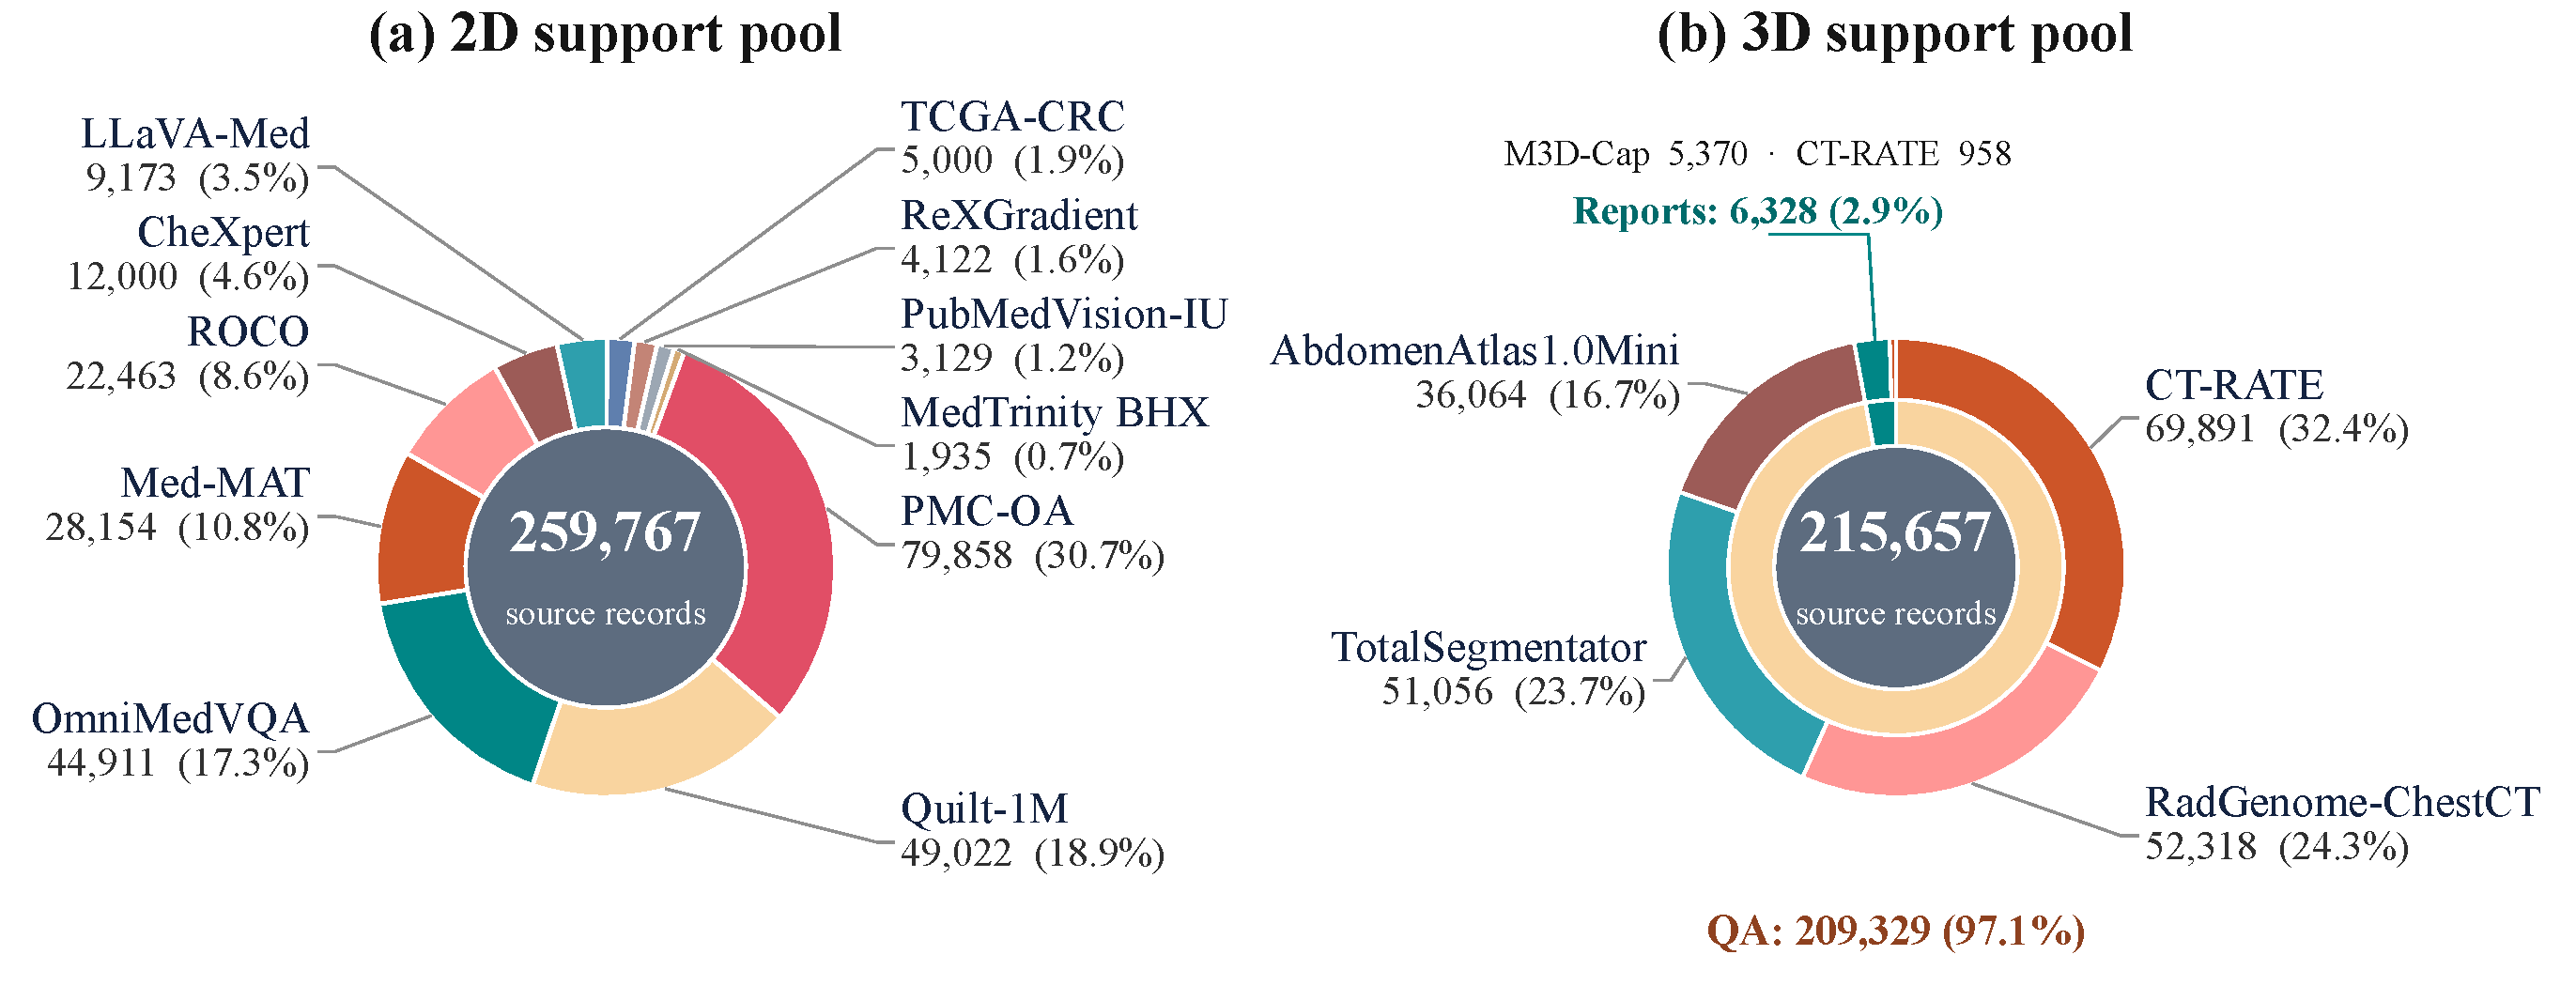
\includegraphics[width=\linewidth]{figures/support_composition.pdf}
\caption{Support-source composition. (a) The 2D support pool contains 259,767 source records. (b) The 3D support pool contains 215,657 source records: the inner ring separates question--answer pairs and reports, and the outer ring identifies their sources. Sector areas and percentages are relative to the total in each panel.}
\label{fig:support_composition}
\end{figure}

\begin{table}[htb]
\centering\small
\caption{Official resources for the support sources. Links for PubMedVision-IU, MedTrinity BHX, and TCGA-CRC lead to their parent datasets.}
\label{tab:support_links}
\setlength{\tabcolsep}{4pt}
\def\UrlFont{\footnotesize\sffamily}
\def\UrlBigBreaks{}
\begin{tabularx}{\linewidth}{@{}L{.28\linewidth}Y@{}}
\toprule
Dataset & Official resource\\
\midrule
\multicolumn{2}{@{}l}{\textit{2D support}}\\
PMC-OA\newline\citep{lin2023pmcclip} & \url{https://weixionglin.github.io/PMC-CLIP/}\\
Quilt-1M\newline\citep{ikezogwo2023quilt} & \url{https://github.com/wisdomikezogwo/quilt1m}\\
OmniMedVQA\newline\citep{hu2024omnimedvqa} & \url{https://github.com/OpenGVLab/Multi-Modality-Arena}\\
Med-MAT\newline\citep{cai2025medmat} & \url{https://github.com/FreedomIntelligence/Med-MAT}\\
ROCO\newline\citep{pelka2018roco} & \url{https://github.com/razorx89/roco-dataset}\\
CheXpert\newline\citep{irvin2019chexpert} & \url{https://aimi.stanford.edu/datasets/chexpert-chest-x-rays}\\
LLaVA-Med\newline\citep{li2023llava} & \url{https://github.com/microsoft/LLaVA-Med}\\
TCGA-CRC\newline\citep{tcga2012colorectal} & \url{https://gdc.cancer.gov/about-data/publications/coadread_2012}\\
ReXGradient\newline\citep{zhang2025rexgradient} & \url{https://huggingface.co/datasets/rajpurkarlab/ReXGradient-160K}\\
PubMedVision-IU subset\newline\citep{chen2024pubmedvision} & \url{https://huggingface.co/datasets/FreedomIntelligence/PubMedVision}\\
MedTrinity BHX\newline\citep{xie2025medtrinity} & \url{https://github.com/UCSC-VLAA/MedTrinity-25M}\\
\midrule
\multicolumn{2}{@{}l}{\textit{3D support}}\\
AbdomenAtlas1.0Mini\newline\citep{li2024abdomenatlas} & \url{https://huggingface.co/datasets/AbdomenAtlas/AbdomenAtlas1.0Mini}\\
CT-RATE\newline\citep{hamamci2026ctrate} & \url{https://huggingface.co/datasets/ibrahimhamamci/CT-RATE}\\
RadGenome-ChestCT\newline\citep{zhang2025radgenome} & \url{https://huggingface.co/datasets/RadGenome/RadGenome-ChestCT}\\
TotalSegmentator\newline\citep{wasserthal2023totalsegmentator} & \url{https://github.com/wasserth/TotalSegmentator}\\
M3D-Cap\newline\citep{bai2024m3d} & \url{https://huggingface.co/datasets/GoodBaiBai88/M3D-Cap}\\
\bottomrule
\end{tabularx}
\end{table}
